\chapter{Resultados Numéricos}\visiblelbl{chap:resultados}

Testamos nossa implementação com a interface de testes CUTEr, utilizando 767
problemas com variáveis ou restrições da ordem de até $10^6$.
Esses problemas são aqueles cujos arquivos 
SIF, específicos do CUTEr, utilizados para descrever o
problema, são considerados pequenos.
Não utilizamos problemas com variáveis fixas, pois ainda não
temos uma versão estável com essa implementação.

O nosso algoritmo foi aplicado sequencialmente a cada problema, utilizando um
máximo de $2\times10^5$ iterações e restaurações, e 2 horas de tempo de
execução. 
Os possíveis resultados para a execução do algoritmo são
\begin{description}
  \item[Convergiu:] Indica que o algoritmo encontrou um ponto estacionário para o
    problema de minimização.
  \item[Estacionário da Infactibilidade: ] O algoritmo encontrou um ponto
    infactível estacionário para o problema de infactibilidade.
  \item[Máximo de Iterações:] Indica que o algoritmo efetuou o número máximo de
    iterações permitidas, mas não convergiu.
  \item[Máximo de Restaurações:] Indica que o algoritmo efetuou o número máximo de
    restaurações permitidas mas não conseguiu encontrar um ponto $z_c^k$ dentro
    do cilindro de raio $\rho$.
  \item[$\rhomax$ pequeno:] Indica que $\rhomax$ ficou muito pequeno.
    Isso sugere que os passos tangentes não fizeram progresso suficiente.
  \item[Limite de Tempo:] Indica que o algoritmo atingiu o máximo de tempo
    permitido, mas não encontrou um ponto estacionário.
  \item[Ilimitado:] Indica que o algoritmo encontrou algum ponto com norma maior
    que $10^{10}$.  
  \item[Falha:] Indica que o algoritmo teve algum problema imprevisto, como falta
    de memória.
\end{description}
Um resumo dos resultados está na Tabela \ref{tab:summary}.
A lista completa dos resultados do algoritmo pode ser encontrada no Apêndice
\ref{chap:results}.
%2013.04.17
\begin{table}[!ht]
  \centering
  \begin{tabular}{|l||r|r|} \hline
    \multirow{2}{*}{\bf ExitFlag} &
    \multicolumn{2}{|c|}{\bf Total} \\ \cline{2-3}
    & {\bf \No} & {\bf \%}
    \\ \hline
    {\bf  Convergiu  } 
    & 689  &  89.60   \\ \hline
    {\bf  Máximo de Iterações  } 
    &   3  &   0.39   \\ \hline
    {\bf  Máximo de Restaurações } 
    &  16  &   2.08   \\ \hline
    {\bf  $\rhomax$ pequeno  } 
    &  23  &   2.99   \\ \hline
    {\bf  Limite de Tempo  } 
    &  14  &   1.82   \\ \hline
    {\bf  Estacionário da Infactibilidade  } 
    &   9  &   1.17   \\ \hline
    {\bf  Ilimitado  } 
    &   3  &   0.39   \\ \hline
    {\bf  Falha  } 
    &  12  &   1.56   \\ \hline
    {\bf  Total  } 
    & 767  & 100.00   \\ \hline
  \end{tabular}
  \caption{Resumo dos resultados} 
  \label{tab:summary}
\end{table}

Separamos os testes em quatro conjuntos em função do tipo de restrições:
os irrestritos; os que têm apenas restrições de igualdade;
os que tem apenas restrições de desigualdade;
e os que tem restrições dos dois tipos.
As tabelas \ref{tab:unc}, \ref{tab:equ}, \ref{tab:ineq} e \ref{tab:gencon}
mostram os resultados para cada um desses conjuntos, respectivamente.

\begin{table}[!ht]
\centering
\begin{tabular}{|c||c|c|} \hline
\multirow{2}{*}{\bf Sa\'ida do Algoritmo} &
\multicolumn{2}{|c|}{\bf Irrestritos} \\ \cline{2-3}
& {\bf \No} & {\bf \%}
\\ \hline
{\bf  Convergiu  } 
& 230  &  94.26  \\ \hline
{\bf  M\'aximo de Itera\c{c}\~oes  } 
&   2  &   0.82  \\ \hline
{\bf  M\'aximo de Restaura\c{c}\~oes  } 
&   0  &   0.00  \\ \hline
{\bf  $\rhomax$ pequeno  } 
&   2  &   0.82  \\ \hline
{\bf  Limite de Tempo  } 
&   5  &   2.05  \\ \hline
{\bf  Estacion\'ario da Infactibilidade  } 
&   0  &   0.00  \\ \hline
{\bf  Ilimitado  } 
&   1  &   0.41  \\ \hline
{\bf  Falha  } 
&   4  &   1.64  \\ \hline
{\bf  Total  } 
& 244  & 100.00  \\ \hline
\end{tabular}
\caption{ Resultados do algoritmo para os problemas irrestritos }
\label{tab:unc}
\end{table}
\begin{table}[!ht]
\centering
\begin{tabular}{|c||c|c|} \hline
\multirow{2}{*}{\bf Sa\'ida do Algoritmo} &
\multicolumn{2}{|c|}{\bf Igualdade} \\ \cline{2-3}
& {\bf \No} & {\bf \%}
\\ \hline
{\bf  Convergiu  } 
& 221  &  85.33  \\ \hline
{\bf  M\'aximo de Itera\c{c}\~oes  } 
&   1  &   0.39  \\ \hline
{\bf  M\'aximo de Restaura\c{c}\~oes  } 
&   9  &   3.47  \\ \hline
{\bf  $\rhomax$ pequeno  } 
&  14  &   5.41  \\ \hline
{\bf  Limite de Tempo  } 
&   5  &   1.93  \\ \hline
{\bf  Estacion\'ario da Infactibilidade  } 
&   5  &   1.93  \\ \hline
{\bf  Ilimitado  } 
&   2  &   0.77  \\ \hline
{\bf  Falha  } 
&   2  &   0.77  \\ \hline
{\bf  Total  } 
& 259  & 100.00  \\ \hline
\end{tabular}
\caption{ Resultados do algoritmo para os problemas de igualdade }
\label{tab:equ}
\end{table}
\begin{table}[!ht]
\centering
\begin{tabular}{|c||c|c|} \hline
\multirow{2}{*}{\bf Sa\'ida do Algoritmo} &
\multicolumn{2}{|c|}{\bf Desigualdade} \\ \cline{2-3}
& {\bf \No} & {\bf \%}
\\ \hline
{\bf  Convergiu  } 
& 186  &  92.08  \\ \hline
{\bf  M\'aximo de Itera\c{c}\~oes  } 
&   0  &   0.00  \\ \hline
{\bf  M\'aximo de Restaura\c{c}\~oes  } 
&   5  &   2.48  \\ \hline
{\bf  $\rhomax$ pequeno  } 
&   3  &   1.49  \\ \hline
{\bf  Limite de Tempo  } 
&   2  &   0.99  \\ \hline
{\bf  Estacion\'ario da Infactibilidade  } 
&   4  &   1.98  \\ \hline
{\bf  Ilimitado  } 
&   0  &   0.00  \\ \hline
{\bf  Falha  } 
&   2  &   0.99  \\ \hline
{\bf  Total  } 
& 202  & 100.00  \\ \hline
\end{tabular}
\caption{ Resultados do algoritmo para os problemas de desigualdade }
\label{tab:ineq}
\end{table}
\begin{table}[!ht]
\centering
\begin{tabular}{|c||c|c|} \hline
\multirow{2}{*}{\bf Sa\'ida do Algoritmo} &
\multicolumn{2}{|c|}{\bf Rest. Gerais} \\ \cline{2-3}
& {\bf \No} & {\bf \%}
\\ \hline
{\bf  Convergiu  } 
&  52  &  81.25  \\ \hline
{\bf  M\'aximo de Itera\c{c}\~oes  } 
&   0  &   0.00  \\ \hline
{\bf  M\'aximo de Restaura\c{c}\~oes  } 
&   2  &   3.12  \\ \hline
{\bf  $\rhomax$ pequeno  } 
&   4  &   6.25  \\ \hline
{\bf  Limite de Tempo  } 
&   2  &   3.12  \\ \hline
{\bf  Estacion\'ario da Infactibilidade  } 
&   0  &   0.00  \\ \hline
{\bf  Ilimitado  } 
&   0  &   0.00  \\ \hline
{\bf  Falha  } 
&   4  &   6.25  \\ \hline
{\bf  Total  } 
&  64  & 100.00  \\ \hline
\end{tabular}
\caption{ Resultados do algoritmo para os problemas igualdade e desigualdade }
\label{tab:gencon}
\end{table}

Escolhemos comparar nosso algoritmo com IPOPT \cite{bib:ipopt}, 
e o ALGENCAN \cite{bib:algencan1,bib:algencan2}, dois métodos bastante
competitivos da área.
A comparação foi feita utilizando o conceito de perfil de desempenho definido
por \citet{bib:performance-profile}.
Considerando um conjunto $S$ de algoritmos aplicados à um conjunto $P$ de
problemas, definimos a razão de desempenho como
$$r_{p,s} = \frac{t_{p,s}}{\min\{t_{p,s} : s \in S\}},$$
para cada $p\in P$ e $s \in S$, onde $t_{p,s}$ é o tempo gasto pelo algoritmo
$s$ para resolver o problema $p$.
O desempenho do algoritmo, em comparação ao conjunto de algoritmos considerado, 
é dado pela função 
$$\mathcal{P}_s(t) = \frac{1}{N_p} \vert\{p \in P : r_{p,s} \leq t\}\vert,$$
onde $N_p$ é o número de problemas, isto é, a cardinalidade de $P$.
Se um algoritmo $s$ não consegue resolver o problema $p$, definimos $r_{p,s} =
\infty$. 
Também definimos o maior valor finito para o qual os algoritmos convergem como
$$r_f = \max_{p,s}\{r_{p,s} : r_{p,s} < \infty\}.$$
O valor para $\infty$ computacionalmente depende da implementação. Nós
utilizamos a linguagem Python e o valor \verb+float('inf')+, que se comporta
como o valor simbólico $\infty$.

A função $\mathcal{P}_s(t)$ mede a fração
dos algoritmos resolvidos pelo algoritmo $s$ dentro do tempo $t$ escalado pelo tempo do
algoritmo mais rápido.
Note que, por definição, sempre temos $r_{p,s} \geq 1$, de modo que
o gráfico deve ser desenhado no intervalo $[1,r_f]$.
O valor $\mathcal{P}_s(1)$ indica a eficiência do 
algoritmo $s$, enquanto que o valor $\mathcal{P}_s(r_f)$ indica a robustez.

Os testes foram feitos num notebook Dell XPS 15 L502X, com processador i7-2820QM
2.3 GHz com 8Gb de RAM. 
Consideramos como critério de convergência as infactibilidades dual, primal e a
complementaridade
serem menores que $10^{-6}$, isto é, $\varepsilon_g = \varepsilon_h =
\varepsilon_a = 10^{-6}$ no Algoritmo \ref{alg:outline}; e um máximo de tempo de
execução do algoritmo de 2 horas. Para o IPOPT, utilizamos a versão 3.10.4 com
as opções
\begin{lstlisting}[frame=single]
max_cpu_time 7200
tol 1e-6
constr_viol_tol 1e-6
\end{lstlisting}
Para o ALGENCAN, usamos a versão 2.4.0 com as opções
\begin{lstlisting}[frame=single]
FEASIBILIT 1.0D-6
OPTIMALITY 1.0D-6
\end{lstlisting}
e a execução foi interrompida externamente.
Os parâmetros utilizados na nossa implementação para a realização destes testes
foram
$\epsmu = 10^{-6}$,
$\nu = 1$,
$\alpha_\rho = 100$,
$\alpha_h = 100$,
$\eta_1 = 10^{-3}$,
$\eta_2 = 0.2$,
$\alpha_R = 0.75$,
$\alpha_I = 2.5$,
$\phi_1 = 1$,
$\beta_1 = 0.1$,
$\beta_2 = 0.25$,
$\beta_3 = 0.95$,
$\theta = 0.99995$,
$\varepsilon_1 = 10^{-6}$,
$\varepsilon_2 = 10^{-14}$, e 
$\varepsilon_3 = 10^{-8}$.

%Os algoritmos são comparados com duas considerações diferentes para os problemas
%em que ocorre convergência a pontos estacionários da infactibilidade.
%No que chamamos de comparação rigorosa, convergência a ponto estacionário da
%infactibilidade é considerada como falha, e a na comparação não rigorosa, aceitamos
%os pontos estacionários da infactibilidade como um resultado positivo.
A Figura \ref{fig:cuter_strict} mostra o gráfico de perfil de desempenho
do DCICPP, IPOPT e ALGENCAN, para todos os problemas do nosso conjunto.
%, considerando a convergência rigorosa.
%A Figura \ref{fig:cuter_notstrict} mostra o gráfico de perfil de desempenho
%do DCICPP e do IPOPT para todos os problemas, considerando a convergência
%não rigorosa.
%Essas duas figuras indicam 
Essa figura indica que o DCICPP é um método bastante competitivo.
Nosso algoritmo resolve alguns problemas mais rapidamente,
mas o ALGENCAN logo o ultrapassa. O IPOPT demora um pouco mais, mas recupera a
diferença. 
Com o decorrer de 2 horas, nosso algoritmo consegue resolver uma quantidade
maior de problemas que o IPOPT, mas menor que o ALGENCAN.

\begin{figure}[!ht]
\centering
\includegraphics[width=0.9\textwidth]{pdfimgs/cuter_all.pdf}
\caption{ Comparação do DCICPP com o IPOPT e o ALGENCAN nos 767 problemas 
do CUTEr. }
\label{fig:cuter_strict}
\end{figure}

%\begin{figure}[!ht]
%\centering
%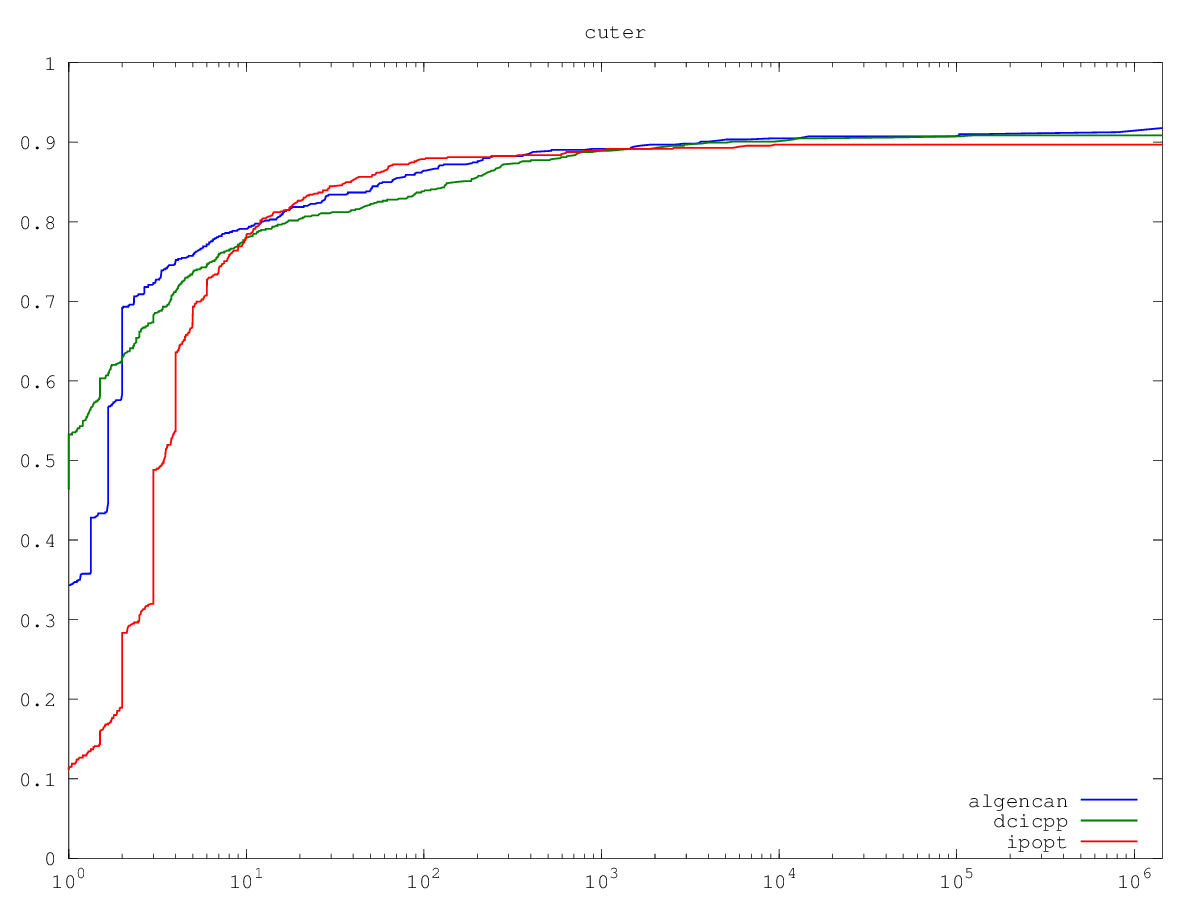
\includegraphics[width=0.9\textwidth]{plots/cuter_notstrict.png}
%\caption{ Comparação do DCICPP com o IPOPT nos problemas pequenos do CUTEr, com
%convergência a pontos estacionários da infactibilidade. }
%\label{fig:cuter_notstrict}
%\end{figure}

Numa tentativa de entender melhor as falhas de nosso algoritmo, fizemos uma
separação do conjunto de problemas, em relação ao tipo de restrições e dos
limitantes da variáveis. Como mostramos na Seção
\ref{sec:cuter_classify}, em função das restrições, os problemas são divididos
em
\begin{itemize}
  \item \verb+unc+ - Problemas irrestritos;
  \item \verb+equ+ - Problemas apenas com restrições de igualdade;
  \item \verb+ineq+ - Problemas apenas com restrições de desigualdade;
  \item \verb+gencon+ - Problemas com restrições de igualdade e
    desigualdade.
\end{itemize}
Para os problemas restritos, podemos ter ainda 
\begin{itemize}
  \item \verb+linear+ - Problemas que contém apenas restrições
    lineares;
  \item \verb+nonlin+ - Problemas com restrições não lineares.
\end{itemize}
Em relação às variáveis, podemos classificar os problemas em
\begin{itemize}
  \item \verb+free+ - Problemas em que nenhuma variável tem limitante.
  \item \verb+lower+ - Problemas em que as variáveis têm apenas limitante
    inferior, ou nenhum limitante.
  \item \verb+upper+ - Problemas em que as variáveis têm apenas limitante
    superior, ou nenhum limitante.
  \item \verb+box+ - Problemas em que existem variáveis com limitante inferior e
    variáveis com limitante superior, podendo haver variáveis com os dois
    limitantes.
\end{itemize}
Separamos os resultados para todas as possíveis combinações de classificação
acima. Infelizmente, algumas destas combinações não são informativas, por conter uma
quantidade muito pequena de testes. No entanto, achamos válido mostrar e
comentar alguns dos resultados. 
%Faremos a análise apenas do caso de convergência rigorosa.

A Figura \ref{fig:union_unc_strict} mostra o gráfico de perfil de desempenho do
DCICPP com o IPOPT e o ALGENCAN para o subconjunto dos problemas irrestritos.
Podemos ver que o DCICPP é superior ao IPOPT nesse conjunto de problema, tanto
em questão de eficiência, quanto de robustez. O ALGENCAN e o DCICPP são
equivalentes.
Note que para esse tipo de problema o método DCICPP é composto apenas pelo passo
tangente, no entanto sem a restrição do espaço nulo. Nesse caso, o método é
basicamente o método de Steihaug com caixas para aproximações quadráticas
sucessivas.

\begin{figure}[!ht]
\centering
\includegraphics[width=0.9\textwidth]{pdfimgs/cuter_unc.pdf}
\caption{ Comparação do DCICPP com o IPOPT e o ALGENCAN para problemas
irrestritos.}
\label{fig:union_unc_strict}
\end{figure}

A Figura \ref{fig:union_equ_strict} mostra o gráfico de perfil de
desempenho do DCICPP com o IPOPT e o ALGENCAN para o subconjunto dos problemas
com restrições apenas de igualdade. O desempenho do DCICPP para esses problemas é
consideravelmente melhor. Podemos ver um alto nível de eficiência, e bastante
competitividade.

\begin{figure}[!ht]
\centering
\includegraphics[width=0.9\textwidth]{pdfimgs/cuter_equ.pdf}
\caption{ Comparação do DCICPP com o IPOPT e o ALGENCAN nos problemas com
restrições apenas de igualdade.}
\label{fig:union_equ_strict}
\end{figure}

A Figura \ref{fig:union_ineq_strict} mostra o gráfico de perfil de
desempenho do DCICPP com o IPOPT e o ALGENCAN para o subconjunto dos problemas
com restrições apenas de desigualdade. Neste subconjunto, apesar de resolvermos
mais problemas em menos tempo, o nosso método fica inferior para uma certa
parcela dos problemas. 

\begin{figure}[!ht]
\centering
\includegraphics[width=0.9\textwidth]{pdfimgs/cuter_ineq.pdf}
\caption{ Comparação do DCICPP com o IPOPT e o ALGENCAN nos problemas com
restrições apenas de desigualdade.}
\label{fig:union_ineq_strict}
\end{figure}

A Figura \ref{fig:union_gencon_strict} mostra o gráfico de perfil de
desempenho do DCICPP com o IPOPT e o ALGENCAN para o subconjunto dos problemas
com restrições de igualdade e de desigualdade. A quantidade de problemas neste
subconjunto é muito pequena para que se possa tirar alguma conclusão definitiva.
Tendo isso em mente, podemos afirmar que os métodos são equivalentes.

\begin{figure}[!ht]
\centering
\includegraphics[width=0.9\textwidth]{pdfimgs/cuter_gencon.pdf}
\caption{ Comparação do DCICPP com o IPOPT e o ALGENCAN nos problemas com
  restrições de igualdade e de desigualdade.}
\label{fig:union_gencon_strict}
\end{figure}

Os resultados mostrados aqui sugerem que nosso método pode render um software
profissional. Alguns ajustes são necessários para expandir sua área de
atuação.
É importante lembrar que esta implementação, assim como o próprio método, foi
iniciada a pouco tempo, e que não é esperado que ela já supere os outros algoritmos
bem estabelecidos.
Com isso em mente, os resultados sugerem que as estratégias descritas aqui são
viáveis e que devem gerar mais projetos de pesquisa.
